% Figure from MATH 591 notes, section 2. Compile with the notes preamble.
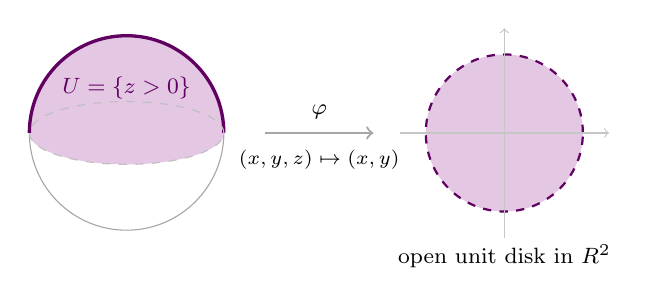
\begin{tikzpicture}[scale=0.95]
\draw[gray!70] (0,0) circle (1.3);
\fill[violet!22] (-1.3,0) arc (180:0:1.3) -- cycle;
\fill[violet!22] (0,0) ellipse (1.3 and 0.42);
\draw[violet!75!black,very thick] (-1.3,0) arc (180:0:1.3);
\draw[gray!50,dashed] (0,0) ellipse (1.3 and 0.42);
\node[violet!75!black,font=\footnotesize] at (0,0.6) {$U=\{z>0\}$};
\draw[->,thick,gray!70] (1.85,0) -- (3.3,0);
\node[font=\footnotesize,above] at (2.575,0.06) {$\varphi$};
\node[font=\scriptsize,below] at (2.575,-0.1) {$(x,y,z)\mapsto(x,y)$};
\begin{scope}[xshift=5.05cm]
\fill[violet!22] (0,0) circle (1.05);
\draw[violet!75!black,thick,dashed] (0,0) circle (1.05);
\draw[gray!45,->] (-1.4,0)--(1.4,0); \draw[gray!45,->] (0,-1.4)--(0,1.4);
\node[font=\footnotesize] at (0,-1.65) {open unit disk in $\mathbb{R}^2$};
\end{scope}
\end{tikzpicture}
